\documentclass[tikz,border=8pt]{standalone}
\usepackage{tikz}
\usetikzlibrary{arrows.meta,calc}

\definecolor{primary}{HTML}{143264}
\definecolor{secondary}{HTML}{8C281E}
\definecolor{tealcol}{HTML}{117A65}
\definecolor{orangecol}{HTML}{C77C02}
\definecolor{greycol}{HTML}{505A64}

\begin{document}
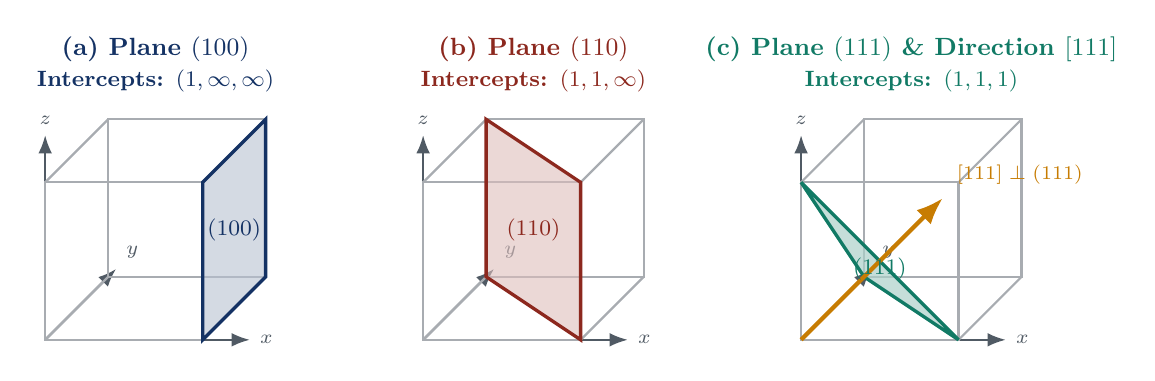
\begin{tikzpicture}[>=Latex]

  % (a) (100) plane
  \begin{scope}[shift={(0,0)}]
    \node[align=center, font=\bfseries\small, text=primary] at (1.4, 3.5) {(a) Plane $(100)$\\ \footnotesize Intercepts: $(1,\infty,\infty)$};
    % Axes
    \draw[->, thick, greycol] (0,0) -- (2.6,0) node[right, font=\scriptsize] {$x$};
    \draw[->, thick, greycol] (0,0) -- (0,2.6) node[above, font=\scriptsize] {$z$};
    \draw[->, thick, greycol] (0,0) -- (0.9,0.9) node[above right, font=\scriptsize] {$y$};
    % Cube wireframe
    \draw[thick, greycol!50] (0,0) -- (2,0) -- (2,2) -- (0,2) -- cycle;
    \draw[thick, greycol!50] (0.8,0.8) -- (2.8,0.8) -- (2.8,2.8) -- (0.8,2.8) -- cycle;
    \draw[thick, greycol!50] (0,0) -- (0.8,0.8) (2,0) -- (2.8,0.8) (2,2) -- (2.8,2.8) (0,2) -- (0.8,2.8);
    % Shaded (100) plane at x = 1 (front face)
    \fill[primary!30, draw=primary, very thick, fill opacity=0.6] 
      (2,0) -- (2.8,0.8) -- (2.8,2.8) -- (2,2) -- cycle;
    \node[font=\footnotesize\bfseries, primary] at (2.4, 1.4) {$(100)$};
  \end{scope}

  % (b) (110) plane
  \begin{scope}[shift={(4.8,0)}]
    \node[align=center, font=\bfseries\small, text=secondary] at (1.4, 3.5) {(b) Plane $(110)$\\ \footnotesize Intercepts: $(1,1,\infty)$};
    % Axes
    \draw[->, thick, greycol] (0,0) -- (2.6,0) node[right, font=\scriptsize] {$x$};
    \draw[->, thick, greycol] (0,0) -- (0,2.6) node[above, font=\scriptsize] {$z$};
    \draw[->, thick, greycol] (0,0) -- (0.9,0.9) node[above right, font=\scriptsize] {$y$};
    % Cube wireframe
    \draw[thick, greycol!50] (0,0) -- (2,0) -- (2,2) -- (0,2) -- cycle;
    \draw[thick, greycol!50] (0.8,0.8) -- (2.8,0.8) -- (2.8,2.8) -- (0.8,2.8) -- cycle;
    \draw[thick, greycol!50] (0,0) -- (0.8,0.8) (2,0) -- (2.8,0.8) (2,2) -- (2.8,2.8) (0,2) -- (0.8,2.8);
    % Shaded (110) diagonal plane
    \fill[secondary!30, draw=secondary, very thick, fill opacity=0.6] 
      (2,0) -- (0.8,0.8) -- (0.8,2.8) -- (2,2) -- cycle;
    \node[font=\footnotesize\bfseries, secondary] at (1.4, 1.4) {$(110)$};
  \end{scope}

  % (c) (111) plane & [111] direction
  \begin{scope}[shift={(9.6,0)}]
    \node[align=center, font=\bfseries\small, text=tealcol] at (1.4, 3.5) {(c) Plane $(111)$ \& Direction $[111]$\\ \footnotesize Intercepts: $(1,1,1)$};
    % Axes
    \draw[->, thick, greycol] (0,0) -- (2.6,0) node[right, font=\scriptsize] {$x$};
    \draw[->, thick, greycol] (0,0) -- (0,2.6) node[above, font=\scriptsize] {$z$};
    \draw[->, thick, greycol] (0,0) -- (0.9,0.9) node[above right, font=\scriptsize] {$y$};
    % Cube wireframe
    \draw[thick, greycol!50] (0,0) -- (2,0) -- (2,2) -- (0,2) -- cycle;
    \draw[thick, greycol!50] (0.8,0.8) -- (2.8,0.8) -- (2.8,2.8) -- (0.8,2.8) -- cycle;
    \draw[thick, greycol!50] (0,0) -- (0.8,0.8) (2,0) -- (2.8,0.8) (2,2) -- (2.8,2.8) (0,2) -- (0.8,2.8);
    % Shaded (111) plane connecting (2,0,0), (0,0.8,0.8), (0,2,0)
    \fill[tealcol!35, draw=tealcol, very thick, fill opacity=0.7] 
      (2,0) -- (0.8,0.8) -- (0,2) -- cycle;
    % Direction vector [111] from origin (0,0,0) perpendicular to plane
    \draw[->, line width=1.5pt, orangecol] (0,0) -- (1.8, 1.8) node[above right=1pt, font=\scriptsize\bfseries] {$[111]\perp(111)$};
    \node[font=\footnotesize\bfseries, tealcol] at (1.0, 0.9) {$(111)$};
  \end{scope}

\end{tikzpicture}
\end{document}
